\documentclass[
	% -- opções da classe memoir --
	12pt,				% tamanho da fonte
	%openright,			% capítulos começam em pág ímpar (insere página vazia caso preciso)
	oneside,			% para impressão em recto e verso. Oposto a oneside
	a4paper,			% tamanho do papel. 
	% -- opções da classe abntex2 --
	%chapter=TITLE,		% títulos de capítulos convertidos em letras maiúsculas
	%section=TITLE,		% títulos de seções convertidos em letras maiúsculas
	%subsection=TITLE,	% títulos de subseções convertidos em letras maiúsculas
	%subsubsection=TITLE,% títulos de subsubseções convertidos em letras maiúsculas
	% -- opções do pacote babel --
	english,			% idioma adicional para hifenização
	french,				% idioma adicional para hifenização
	spanish,			% idioma adicional para hifenização
	brazil,				% o último idioma é o principal do documento
	]{abntex2}


% ---
% PACOTES
% ---

% ---
% Pacotes fundamentais 
% ---
\usepackage{pslatex}			% Usa a fonte Latin Modern
\usepackage[T1]{fontenc}		% Selecao de codigos de fonte.
\usepackage[utf8]{inputenc}		% Codificacao do documento (conversão automática dos acentos)
\usepackage{indentfirst}		% Indenta o primeiro parágrafo de cada seção.
\usepackage{color}				% Controle das cores
\usepackage{graphicx}			% Inclusão de gráficos
\usepackage{microtype} 			% para melhorias de justificação
\usepackage{transparent}
\usepackage{eso-pic}
\usepackage{float}
\usepackage{array}
\usepackage{epstopdf}
\usepackage{url}
\usepackage{amsmath}
\usepackage[
  locale = DE % comma as decimal mark
]{siunitx}
% ---

% ---
% Pacotes adicionais, usados no anexo do modelo de folha de identificação
% ---
\usepackage{multicol}
\usepackage{multirow}
% ---
	
% ---
% Pacotes adicionais, usados apenas no âmbito do Modelo Canônico do abnteX2
% ---
%\usepackage{lipsum}				% para geração de dummy text
% ---

% ---
% Pacotes de citações
% ---
%\usepackage[brazilian,hyperpageref]{backref}	 % Paginas com as citações na bibl
%\usepackage[alf]{abntex2cite}	% Citações padrão ABNT

% --- 
% CONFIGURAÇÕES DE PACOTES
% --- 

% ---
% Configurações do pacote backref
% Usado sem a opção hyperpageref de backref
%\renewcommand{\backrefpagesname}{Citado na(s) página(s):~}
% Texto padrão antes do número das páginas
%\renewcommand{\backref}{}
% Define os textos da citação
%\renewcommand*{\backrefalt}[4]{
%	\ifcase #1 %
%		Nenhuma citação no texto.%
%	\or
%		Citado na página #2.%
%	\else
%		Citado #1 vezes nas páginas #2.%
%	\fi}%
% ---

% ---
% Informações de dados para CAPA e FOLHA DE ROSTO
% ---
\titulo{Engenharia do Trabalho\\Estudo de tempos e métodos em diferentes linhas de montagem}
\autor{Profª Maria de Lourdes Santiago Luz\\Gabriel Rodrigues Munhoz 106802\\Germano Silva Marino 98296\\Guilherme Benetti Martini 107613\\Kaio Vinícius Cervigni Pereira 101580\\João Arthur Pirani Rubio 99859\\Pedro Henrique Friche de Oliveira 94682}
\local{Maringá, Paraná}
\data{Novembro de 2018}
\instituicao{%
  Universidade Estadual de Maringá  - UEM}
\tipotrabalho{Trabalho científico}
% O preambulo deve conter o tipo do trabalho, o objetivo, 
% o nome da instituição e a área de concentração 
\preambulo{"Engenharia: onde os nobres semi-hábeis trabalhadores executam a visão daqueles que imaginam e sonham"}
% ---

% ---
% Configurações de aparência do PDF final

% alterando o aspecto da cor azul
\definecolor{blue}{RGB}{41,5,195}

% informações do PDF
\makeatletter
\hypersetup{
     	%pagebackref=true,
		pdftitle={\@title}, 
		pdfauthor={\@author},
    	pdfsubject={\imprimirpreambulo},
	    pdfcreator={LaTeX with abnTeX2},
		pdfkeywords={abnt}{latex}{abntex}{abntex2}{relatório técnico}, 
		colorlinks=true,       		% false: boxed links; true: colored links
    	linkcolor=blue,          	% color of internal links
    	citecolor=blue,        		% color of links to bibliography
    	filecolor=magenta,      		% color of file links
		urlcolor=blue,
		bookmarksdepth=4
}
\makeatother
% --- 

% --- 
% Espaçamentos entre linhas e parágrafos 
% --- 

% O tamanho do parágrafo é dado por:
\setlength{\parindent}{1.3cm}

% Controle do espaçamento entre um parágrafo e outro:
\setlength{\parskip}{0.2cm}  % tente também \onelineskip

% ---
% compila o indice
% ---
\makeindex
% ---
\usepackage{fancyhdr}
\fancyhead{}
\fancyfoot{}
\lhead{Estudo de tempos e métodos em diferentes linhas de montagem}
\rhead{\thepage}

\AddToShipoutPicture{

\put(0,0){

\parbox[b][\paperheight]{\paperwidth}{%

\vfill

\centering

{\transparent{0.1}
\includegraphics[scale=01.35]{LogoUEM.jpg}}%

\vfill}}}
% ----
% Início do documento
% ----
\begin{document}

\begin{minipage}[c][2cm][c]{3cm} % a primeira minipágina tem uma altura de 1.5cm e uma largura de 3cm.
\centering

\includegraphics[scale=1]{uem-logo.png} 

\end{minipage}

% Seleciona o idioma do documento (conforme pacotes do babel)
%\selectlanguage{english}
\selectlanguage{brazil}

% Retira espaço extra obsoleto entre as frases.
\frenchspacing 

% ----------------------------------------------------------
% ELEMENTOS PRÉ-TEXTUAIS
% ----------------------------------------------------------
%\pretextual

% ---
% Capa
% ---
\imprimircapa
% ---

% ---
% Folha de rosto
% (o * indica que haverá a ficha bibliográfica)
% ---
\imprimirfolhaderosto*

% ---
% inserir o sumario
% ---
\pdfbookmark[0]{\contentsname}{toc}
\tableofcontents*
\newpage

\section[Introdução]{Introdução}
\pagestyle{fancy}

O trabalho consiste em uma cronoanálise da confecção de um barco de papel comparando 3 tipos diferentes de linha de montagem. A primeira sendo operários separados, a segunda em linha de acordo com a melhor eficiencia e a terceira com uma linha desbalanceada já definida, todas com 3 funcionários. Os passos para montagem do barco se encontram na Figura \ref{fig1}.

\begin{figure}[H]
\begin{center}

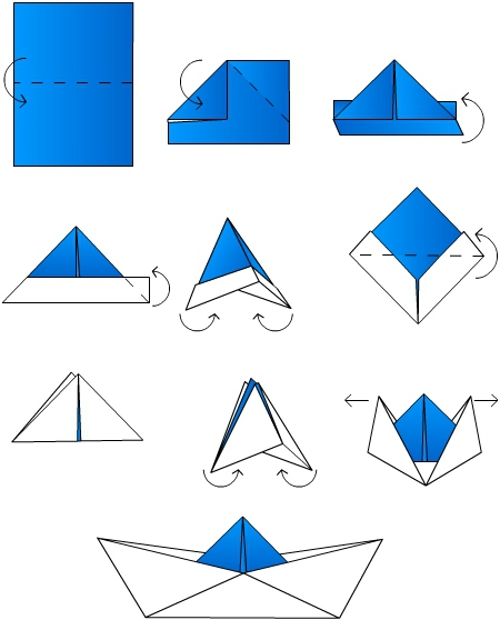
\includegraphics[scale=1]{1.jpg} 

\label{fig1}
\caption{Montagem do barco de papel}
\end{center}
\end{figure}

Foram definidos os tempos padrões para as diversas linhas de montagem e calculados os lead times e takt times de acordo com certa demanda e por fim são comparadas as linhas de montagem. Assim, pode-se obter o resultado da melhor linha de produção e calcular a produtividade de tal de acordo com uma dada jornada de trabalho. Além disso, ainda foram estudadas as curvas de aprendizagem dos operários e discutidos os problemas das linhas.


\newpage
\section[Descrição das linhas de produção]{Descrição das linhas de produção}
\pagestyle{fancy}

Os operários foram separados de acordo com as etapas do processo, sendo que três tipos de processos foram testados e analisados para se calcular o mais eficiente, sendo esses tipos: \\


\begin{minipage}{13cm}
\begin{center}
\textbf{1.} Operários realizando a montagem de todas as etapas do produto individualmente em seu próprio ritmo;\\ 
\textbf{2.} Montagem em linha buscando o máximo de eficiência de acordo com as habilidades de cada operário (balanceada); \\
\textbf{3.} Montagem em linha com as etapas pré-determinadas (desbalanceada).
\end{center}
\end{minipage}\\

A metodologia de produção em linha dividiu o trabalho para os 3 trabalhadores de forma que o primeiro colaborador exercesse as etapas 1, 2 e 3; o segundo as etapas 4 e 5; e o terceiro operador o restante. Já na produção em linha pré-determinada os empregados deveriam realizar as seguintes etapas: 1 e 2 o primeiro operador; 3, 4, 5 e 6 o segundo; 7, 8 e 9 o terceiro.

Durante a avaliação dos processos e analise dos tempos de produção percebeu-se que a produção individual era a menos eficiente, e em linha desbalanceada ficava um pouco mais lenta que em linha balanceada, isso se justifica pelo melhor gestão dos funcionários em relação à suas habilidades nas diferentes etapas do processo, por exemplo a habilidade superior do operário 1 mostrou maior efetividade para realizar as etapas mais complexas em quanto o esforço do operário 2 se comportou melhor em etapas mais simples, enquanto o operário 3 funcionava em qualquer função de forma similar então foi preferido dar deixar a prioridade de escolha das etapas aos outros, utilizando o terceiro para as etapas restantes.


\newpage
\section[Resultados]{Resultados}
\pagestyle{fancy}

Os operadores repetiram a montagem do produto 10 vezes e geraram os tempos contidos na Tabela \ref{tab1}

\begin{table}[H]
\centering
\caption{Tempos durante treinamento dos colaboradores (seg)}
\begin{tabular}{c|c|c|c}

&Tempos do 1º operário	&		Tempos do 2º operário	&		Tempos do 3º operário		\\ \hline
1&	67,1	&		91,3	&		140,3			\\ \hline
2&	67,5	&		117,7		&	127,3			\\ \hline
3&	65,4	&		108,7		&	137,1			\\ \hline
4&	58,3	&		108,9		&	138,8			\\ \hline
5&	67,2	&		122,1		&	95			\\ \hline
6&	59,2	&		117,4		&	132,5			\\ \hline
7&	62,8	&		140,2		&	123,2			\\ \hline
8&	57,3	&		99,9		&	141,3			\\ \hline
9&	67,3	&		109,3		&	108,9			\\ \hline
10	&67,7	&		110,9		&	111,1			\\ \hline
Tempo Médio&	63,98	&		112,64	&		125,55		
	
\label{tab1}
\end{tabular}	
\end{table}
								
O tempo médio de cada operador é dado como o ritmo de cada um. Sendo assim, pode-se notar uma diferença entre os 3 colaboradores, destacando-se o primeiro que detém uma habilidade maior e com isso manteve um ritmo mais constante e mais rápido. Enquanto os dois trabalhadores seguintes mesmo mantendo um ritmo consistente não possuem a técnica certa ou não passaram por treinamento e com isso, geraram um maior tempo médio.

Após a demarcação de todos os tempos com os trabalhadores em linha balanceada e desbalanceada foi possível calcular os tempos médios de cada modelo de produção. Além disso, obteve-se o tempo normal, padrão, lead time, tempo de ciclo, capacidade do processo e takt time segundo certa demanda.

Os tempos obtidos com os colaboradores em linha estão nas tabelas \ref{tab4} e \ref{tab3}.

\begin{table}[H]
\centering
\caption{Tempos com colaboradores em linha balanceada (seg)}
\begin{tabular}{c|c|c|c}

	&Tempos do 1º operário	&		Tempos do 2º operário		&	Tempos do 3º operário	\\ \hline
1&	18,7	&		20,3	&		10,7		\\ \hline
2&	17,9	&		22,8	&		12,1		\\ \hline
3&	18,3	&		22,7	&		13,6		\\ \hline
4&	19,1	&		21,2	&		14,1		\\ \hline
5&	17		&	20,6		&	14		\\ \hline
6&	19,6	&		19,8	&		15		\\ \hline
7&	15		&	19,2		&	14,1		\\ \hline
8&	17,3	&		19,8	&		13,2		\\ \hline
9	&16,5	&		21,6	&		13,3		\\ \hline
10&	17,5	&		21,9	&		12,1		\\ \hline
Tempo Médio	&17,69		&	20,99		&	13,22		
									

\label{tab4}
\end{tabular}	
\end{table}

\begin{table}[H]
\centering
\caption{Tempos com colaboradores em linha desbalanceada (seg)}
\begin{tabular}{c|c|c|c}

	&Tempos do 1º operário		&	Tempos do 2º operário	&		Tempos do 3º operário		\\ \hline
1&	13,38		&	38,6	&		6,06		\\ \hline
2	&14,53		&	36,93		&	8,2		\\ \hline
3	&12,80		&	35,71	&		6,72		\\ \hline
4	&12,39		&	37,58	&		7,97		\\ \hline
5	&15,41		&	35,26	&		5,74		\\ \hline
6	&15,05		&	38,94	&		5,28 \\ \hline
7	&15,05		&	35,49	&		6,52		\\ \hline
8	&15,04		&	36		&	7,69		\\ \hline
9	&14,02		&	36,14	&		6,23		\\ \hline
10	&14,86		&	37,74	&		5,99		\\ \hline
Tempo Médio&	14,25		&	36,84		&	6,64		
									
\label{tab3}
\end{tabular}	
\end{table}

\subsection{Tempo médio e confiabilidade}

O tempo médio foi encontrado com a média aritmética dos tempos apresentados anteriormente e os resultados foram de:

\begin{table}[H]
\centering
\caption{Tempo médio para confecção de um barco (seg)}
\begin{tabular}{c|c|c|c}
&Separados & Em linha balanceada & Em linha desbalanceada \\ \hline
Tempo Médio&	100,73		&	51,9		&	57,73		
									
\label{tab5}
\end{tabular}	
\end{table}

A confiabilidade, no entanto, advém da fórmula:

\begin{center}
\begin{equation}
$$$n=\left(\frac{Z.R}{E.d.x}\right)^2$$$
\end{equation}
\end{center}

n= número de vezes que deveria ser repetida a operação para se ter confiabilidade; Z= coeficiente de acordo com número de repetições; R= amplitude do sistema; E= erro agregado; d= coeficiente de acordo com número de repetições; x= valor médio das variáveis.

Com isso, obteve-se os seguintes resultados para n:

\begin{table}[H]
\centering
\caption{Números de repetições que deveriam ser realizadas}
\begin{tabular}{c|c|c|c}

	&Operador 1&Operador 2&Operador 3 \\ \hline
	Separados	& 6,58 	& 29,04 &	 30,61 \\ \hline
	Em linha balanceada &	 9,57 &	 8,20 	& 17,24 \\ \hline
	Em linha desbalanceada	& 5,84 &	 1,25 &	 18,66 


\label{tab6}
\end{tabular}	
\end{table}

Nota-se que boa parte dos resultados não são confiáveis pois necessitam de mais de 10 repetições, nesse caso seria necessário realizar novas demarcações de tempo para que o resultado seja considerado confiável. É importante salientar que quanto maior a amplitude dos dados mais repetições terão que ser realizadas, pois o grau de eficiencia é baixo.
									

\subsection{Tempo normal e padrão}

O tempo normal, basicamente, é a relação entre o tempo médio que cada operário realiza a atividade com o ritmo com que esse operário trabalha. Sendo aplicado pela seguinte forma:

\begin{equation}
Tn=Tm.k
\end{equation}

Tn= tempo normal; Tm= tempo médio; k= coeficiente gerado do Westinghouse;

	Na aplicação do tempo normal existem diversos fatores de avaliação, como por exemplo: desempenho do ritmo e avaliação objetiva por elementos. Existem também alguns sistemas de avaliação. Um dos sistemas mais utilizados é o Sistema de Westinghouse, que se baseia a partir de 4 fatores: habilidade, esforço, condições e consistência.
	
	Então, o método de Westinghouse foi utilizado para descrever cada operador, mediante a sua habilidade e força, com isso, foi gerado um coeficiente para cada operário de acordo com a Tabela \ref{tab2}.
	
\begin{table}[H]
\centering
\caption{Coeficientes de Westinghouse}
\begin{tabular}{c|c|c|c}


	& 1º operário	&		2º operário		&	3º operário		\\ \hline
Habilidade &	0,11	&		-0,05	&		-0,05		\\ \hline
Condições &	-0,03	&		-0,03	&		-0,03		\\ \hline
Esforço &	0	&		0,08	&		0,05		\\ \hline
Consistência &	0,03	&		-0,02	&		-0,02		\\ \hline
Soma &	0,11	&		-0,02	&		-0,05	
	
\label{tab2}
\end{tabular}	
\end{table}

Os tempos normais calculados se encontram na Tabela \ref{tab8}.

\begin{table}[H]
\centering
\caption{Tempos normais (seg)}
\begin{tabular}{c|c|c|c}


	&1º operário&			2º operário	&		3º operário		\\ \hline
Separado&	67,78	&		116,73		&	116,57		\\ \hline
Em linha balanceada&	19,65	&		20,48	&		11,66	\\ \hline	
Em linha desbalanceada&	15,67	&		36,57		&	6,67		\\ \hline
Tempo normal total&	301,07	&		51,79		&	58,91		
													
\label{tab8}
\end{tabular}	
\end{table}				
							
O tempo padrão nada mais é do que o tempo necessário para se realizar uma operação de acordo com método estabelecido, o operador deve estar apto e treinado, trabalhando todas as horas da jornada de trabalho em ritmo normal.

Para a descoberta do tempo padrão, existem também algumas variáveis que influenciam ele, como por exemplo, quando se tem um operário que não tem tanta habilidade, o tempo padrão sobe, pois acaba tendo uma margem de erro maior, agora ao contrario se o operário for preciso, o tempo padrão automaticamente diminui, pois neste caso quase não vai ter margem de erro. Outra variável que pode ser citada é o clima no ambiente de trabalho, se o clima for agradável, o tempo padrão também abaixa, ao contrario disso se o clima for desagradável, o operário estará mais propicio a erros e consequentemente o tempo padrão aumentará.
A formula para aplicação do tempo padrão é dada por: 

\begin{equation}
Tp=k.Tn
\end{equation}

Tp= tempo padrão; K= fator de tolerância; Tn= tempo normal;

Na confecção dos barquinhos, foi utilizado um fator de tolerância de apenas 6$\%$, pois a atividade é uma atividade monótona e com muitos movimentos repetitivos, porém não exige um grande esforço físico e o ambiente em si estava agradável. Assim, os tempos padrões resultantes foram organizados na Tabela \ref{tab9}.

\begin{table}[H]
\centering
\caption{Tempos padrões (seg)}
\begin{tabular}{c|c|c|c}

	&1º operário	&		2º operário	&		3º operário		\\ \hline
Separado&	71,84	&		123,73	&		123,56		\\ \hline
Em linha balanceada&	20,83	&		21,71	&		12,36		\\ \hline
Em linha desbalanceada&	16,61&			38,77	&		7,07		\\ \hline
Tempo padrão total	&319,13			&54,89	&		62,45							
											
\label{tab9}
\end{tabular}	
\end{table}		

\subsection{Lead time, tempo de ciclo e takt time}

O lead time de uma operação consiste no tempo total desde o início até a finalização. Com isso, pode-se perceber que é o tempo mais completo, pois engloba tanto o tempo da fabricação como também o tempo das movimentações e finalizações.

\begin{table}[H]
\centering
\caption{Lead times (seg)}
\begin{tabular}{c|c|c|c}

	&Separados & Em linha balanceada & Em linha desbalanceada \\ \hline
1 Produto & 72,47& 55,13 &62,47 \\ \hline
Lote de 10 produtos & 724,67& 247,07 &413,62
	
\label{tab7}
\end{tabular}	
\end{table}


Comparando o lead time de 3 operários em relação a apenas um em treinamento é possível notar que há uma discrepância em torno de 20seg. A partir desse fato é notório que o plano de produção siga a metodologia de produção em linha, pois gera uma produtividade maior.

O tempo de ciclo, no entanto, é o tempo de "cuspida", ou seja, após a máquina ou os operadores pegarem ritmo é o tempo que conseguem produzir um novo barco. Tal intervalo de tempo é igual ao gargalo do processo já que é o maior período de tempo durante a fabricação.

\begin{table}[H]
\centering
\caption{Tempo de ciclo (seg)}
\begin{tabular}{c|c|c|c}

	&	Separados	&		Em linha balanceada	&		Em linha desbalanceada		\\ \hline
1 Produto	&123,73		&	21,71	&		38,77					

	
\label{tab10}
\end{tabular}	
\end{table}

O takt time, no entanto, é referente ao tanto de tempo que a empresa possui para gerar um produto para que consiga atender toda sua demanda mensal ou semanal. Assim, para uma demanda de 2500 barcos e com uma jornada de trabalho de 48,75 min/h em 8h diárias, temos que:

Takt time = $\frac{390x60}{2500}$

O takt time para tal demanda foi de 9,36seg.

\subsection{Capacidade}

A capacidade de uma empresa é o tanto que ela consegue produzir em um dado intervalo de tempo. Para calcular a capacidade é necessário saber o tempo de ciclo e o tempo de trabalho sem intervalos. Assim, é possível dividir os dois e quantificar o tamanho da produção que pode ser confeccionada em um dia.

$Cap_1$ = $\frac{6,5x60x60}{21,71}$ = 1077,8 barcos \quad	$Cap_2$ = $\frac{6,5x60x60}{38,77}$ = 603,5 barcos

A primeira capacidade é em relação à linha de produção balanceada e a segunda em relação à desbalanceada. Pode-se notar que a capacidade da empresa muda completamente por causa de uma separação errônea de atividades para cada operário em linha. 

%\subsection{Tempo padrão com finalização}



\newpage
\section[Conclusão]{Conclusão}
\pagestyle{fancy}

Os resultados são bem expressivos e nos mostram que uma produção por linha é mais eficiente que trabalhadores separados e que uma linha desbalanceada cria um gargalo que prejudica muito na produção, pois mesmo que o tempo padrão total seja similar ao de uma linha balanceada a capacidade da empresa é feita com base no tempo de ciclo e isso faz com que haja uma grande diferença entre a linha balanceada e a desbalanceada.

Além disso, foi possível notar que o processo de gestão vai além de cálculos frios e apenas números, já que durante a organização da linha de montagem balanceada foi necessário denotar as etapas condizente com as habilidades de cada operador, para que assim o gargalo da operação ficasse menor.

Em relação aos cálculos nota-se que os tempos padrões tendem a aumentar sempre que os operadores estão inseridos em atividades monótonas, que precisam de certa habilidade, em locais não tão propícios e entre outros fatores. Tudo pode alterar a produtividade de uma indústria, cabe ao engenheiro responsável ponderar quais são os fatores que mais influenciam e diminuir sua influência na linha de produção.
%\bibliographystyle{ieeetr}
%\bibliography{•}

\end{document}
